% chktex-file 1
% chktex-file 29

\FILENAME

\chapter{Introduction to Kubernetes}
\index{Kubernetes}

\section{Topics Covered and Learning Outcome}

\begin{itemize}
\item What is Kubernetes?
\item What are containers?
\item Cluster components in Kubernetes
\item Basic Units in Kubernetes
\item Run an example with Minikube
\item Interactive online tutorial
\item Have a solid understanding of Containers and Kubernetes
\item Understand the CLuster components of Kubernetes
\item Understand the terminology of Kubernetes
\item Gain practical experience with kubernetes
\item With minikube
\item With an interactive online tutorial
\end{itemize}

\section{What is Kubernetes?}

Kubernetes is an open-source platform designed to automate deploying,
scaling, and operating application containers.
\url{https://kubernetes.io/docs/concepts/overview/what-is-kubernetes/}

With Kubernetes, you can:

\begin{itemize}

\item Deploy your applications quickly and predictably.
\item Scale your applications on the fly.
\item Roll out new features seamlessly.
\item Limit hardware usage to required resources only.
\item Run applications in public and private clouds.
\end{itemize}

Kubernetes is

\begin{itemize}

\item Portable: public, private, hybrid, multi-cloud
\item Extensible: modular, pluggable, hookable, composable
\item Self-healing: auto-placement, auto-restart, auto-replication,
  auto-scaling
\end{itemize}

\section{What are containers?}

\begin{figure}[htbp]
\centering
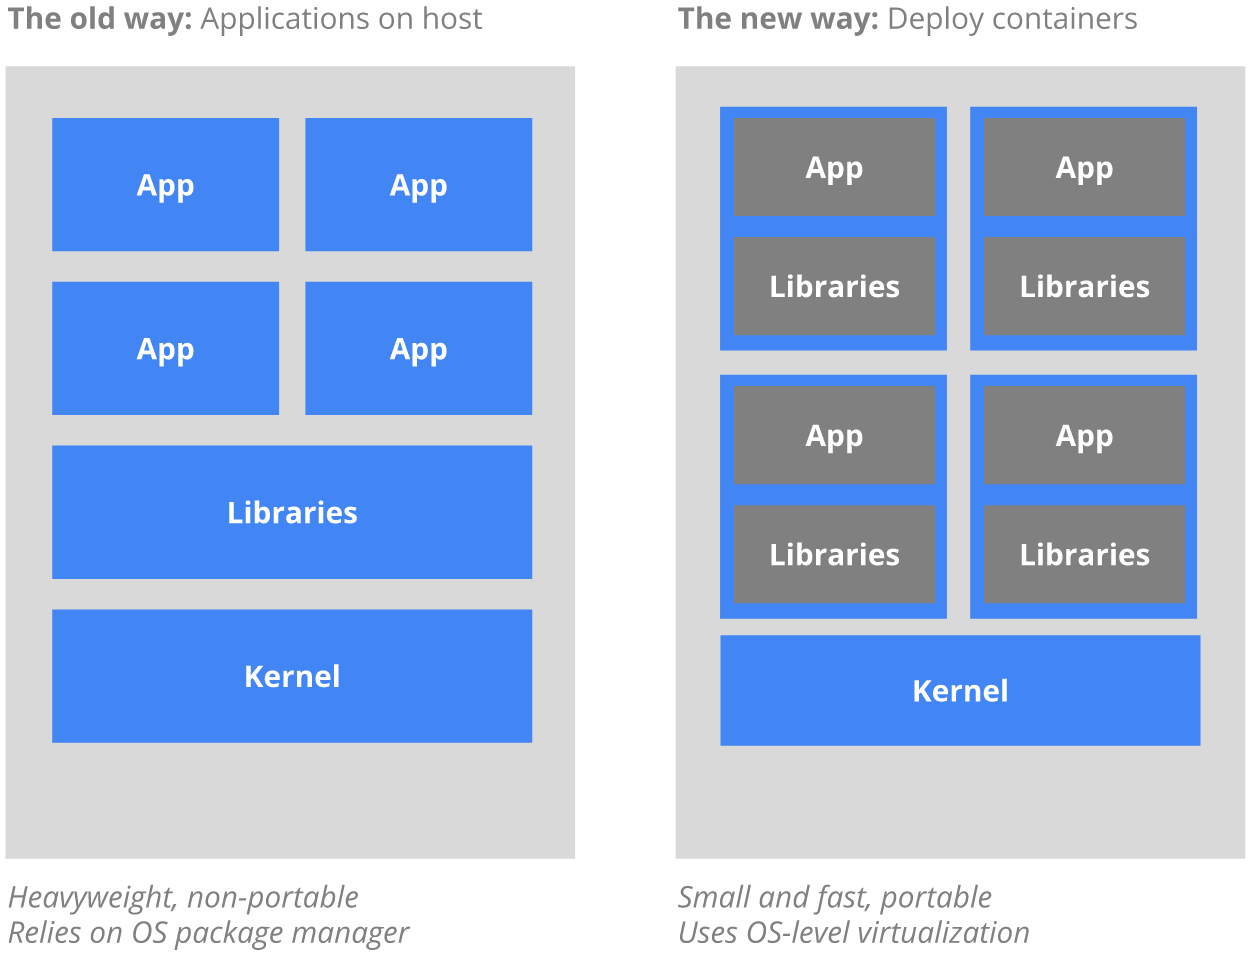
\includegraphics[width=0.8\textwidth]{why_containers.png}
\caption{Kubernetes Containers}
\end{figure}

Image source:

\URL{https://d33wubrfki0l68.cloudfront.net/e7b766e0175f30ae37f7e0e349b87cfe2034a1ae/3e391/images/docs/why_containers.svg}

\section{Terminology}

\begin{description}

\item[Pods:]\index{Pods} A pod (as in a pod of whales or pea pod) is a
  group of one or more containers (such as Docker containers), with
  shared storage/network, and a specification for how to run the
  containers. A pod's contents are always co-located and co-scheduled,
  and run in a shared context. A pod models an application-specific
  \textit{logical host}. It contains one or more application
  containers which are relatively tightly coupled. In a pre-container
  world, they would have executed on the same physical or virtual
  machine.

\item[Services:]\index{Kuberneted!Services} Service is an abstraction
  which defines a logical set of Pods and a policy by which to access
  them. Sometimes they are called a micro-service. The set of Pods
  targeted by a Service is (usually) determined by a Label Selector.

\item[Deployments:]\index{Kuberneted!Deplyments} A Deployment
  controller provides declarative updates for Pods and
  ReplicaSets. You describe a desired state in a Deployment object,
  and the Deployment controller changes the actual state to the
  desired state at a controlled rate. You can define Deployments to
  create new ReplicaSets, or to remove existing Deployments and adopt
  all their resources with new Deployments.

\end{description}

\section{Minikube}
\index{Kubernetes!Minikube}

\begin{enumerate}
\item minikube installation
\item minikube hello-minikube
\end{enumerate}

\subsection{Install minikube}

\paragraph{OSX}\label{osx}

\begin{lstlisting}[language=bash]
curl -Lo minikube https://storage.googleapis.com/minikube/releases/v0.25.0/minikube-darwin-amd64 && chmod +x minikube && sudo mv minikube /usr/local/bin/
\end{lstlisting}

\paragraph{Windows 10}\label{windows-10}

We assume that you have installed Oracle VirtualBox in your machine
which must be a version 5.x.x.

Initially, we need to download two executables.

\href{http://storage.googleapis.com/kubernetes-release/release/v1.4.0/bin/windows/amd64/kubectl.exe}{Download
Kubectl}

\href{https://storage.googleapis.com/minikube/releases/v0.25.0/minikube-windows-amd64.exe}{Download
Minikube}

After downloading these two executables place them in the cloudmesh
directory we earlier created. Rename the \verb|minikube-windows-amd64.exe|
to \verb|minikube.exe|. Makesure minikube.exe and kubectl.exe lie in the
same directory.

\paragraph{Linux}\label{linux}

\begin{lstlisting}[language=bash]
curl -Lo minikube https://storage.googleapis.com/minikube/releases/v0.25.0/minikube-linux-amd64 && chmod +x minikube && sudo mv minikube /usr/local/bin/
\end{lstlisting}

Installing KVM2 is important for Ubuntu distributions

\begin{lstlisting}[language=bash]
$ sudo apt install libvirt-bin qemu-kvm
$ sudo usermod -a -G libvirtd $(whoami)
$ newgrp libvirtd
\end{lstlisting}

We are going to run minikube using KVM2 libraries instead of virtualbox
libraries for windows installation.

Then install the drivers for KVM2,

\begin{lstlisting}[language=bash]
$ curl -LO https://storage.googleapis.com/minikube/releases/latest/docker-machine-driver-kvm2 && chmod +x docker-machine-driver-kvm2 && sudo mv docker-machine-driver-kvm2 /usr/bin/
\end{lstlisting}
%$

\subsection{Start a cluster using Minikube}

\paragraph{OSX Minikube Start}

\begin{lstlisting}[language=bash]
$ minikube start
\end{lstlisting}
%$

\paragraph{Ubuntu Minikube Start}

\begin{lstlisting}[language=bash]
minikube start --vm-driver=kvm2
\end{lstlisting}

\paragraph{Windows 10 Minikube Start}

In this case you must run Windows PowerShell as administrator. For
this search for the application in search and right click and click Run
as administrator. If you are an administrator it will run automatically
but if you are not please make sure you provide the admin login
information in the pop up.

\begin{lstlisting}[language=bash]
$ cd  C:\Users\<username>\Documents\cloudmesh
$ .\minikube.exe start --vm-driver="virtualbox"
\end{lstlisting}

\subsection{Create a deployment}

\begin{lstlisting}[language=bash]
$ kubectl run hello-minikube --image=k8s.gcr.io/echoserver:1.4 --port=8080
\end{lstlisting}

\subsection{Expose the service}

\begin{lstlisting}[language=bash]
$ kubectl expose deployment hello-minikube --type=NodePort
\end{lstlisting}

\subsection{Check running status}

This step is to make sure you have a pod up and running.

\begin{lstlisting}[language=bash]
$ kubectl get pod
\end{lstlisting}

\subsection{Call service api}

\begin{lstlisting}[language=bash]
$ curl $(minikube service hello-minikube --url)
\end{lstlisting}

\subsection{Take a look from Dashboard}

\begin{lstlisting}[language=bash]
$ minikube dashboard
\end{lstlisting}

If you want to get an interactive dashboard,

\begin{lstlisting}[language=bash]
$ .\minikube.exe dashboard --url=true
http://192.168.99.101:30000
\end{lstlisting}

Browse to http://192.168.99.101:30000 in your web browser and it will
provide a GUI dashboard regarding minikube.

\subsection{Delete the service and deployment}

\begin{lstlisting}[language=bash]
$ kubectl delete service hello-minikube
$ kubectl delete deployment hello-minikube
\end{lstlisting}

\subsection{Stop the cluster}

For all platforms we can use the following command.

\begin{lstlisting}[language=bash]
$ minikube stop
\end{lstlisting}

\section{Interactive Tutorial Online}

\begin{itemize}

\item
  Start cluster
  https://kubernetes.io/docs/tutorials/kubernetes-basics/cluster-interactive/
\item
  Deploy app
  https://kubernetes.io/docs/tutorials/kubernetes-basics/cluster-interactive
\item
  Explore
  https://kubernetes.io/docs/tutorials/kubernetes-basics/explore-intro/
\item
  Expose
  https://kubernetes.io/docs/tutorials/kubernetes-basics/expose-intro/
\item
  Scale
  https://kubernetes.io/docs/tutorials/kubernetes-basics/scale-intro/
\item
  Update
  https://kubernetes.io/docs/tutorials/kubernetes-basics/update-interactive/
\item
  MiniKube
  https://kubernetes.io/docs/tutorials/stateless-application/hello-minikube/
\end{itemize}
